
\newcommand{\spina}[3]{
\draw (#1, #2) circle [radius=0.22];
\node at (#1, #2-0.4) {\scriptsize #3};
}
\newcommand{\spinb}[3]{
\draw (#1, #2) circle [radius=0.22];
\node at (#1, #2+0.4) {\scriptsize #3};
}
\newcommand{\spin}[2]{
\draw (#1, #2) circle [radius=0.22];
}
\newcommand{\interact}[2]{
\draw (#1-0.2, #2-0.2) rectangle (#1+0.2, #2+0.2);
}
\newcommand{\upright}[2]{
\draw [->] (#1+0.25,#2+0.25) -- (#1+0.75,#2+0.75);
}
\newcommand{\upleft}[2]{
\draw [->] (#1-0.25,#2+0.25) -- (#1-0.75,#2+0.75);
}
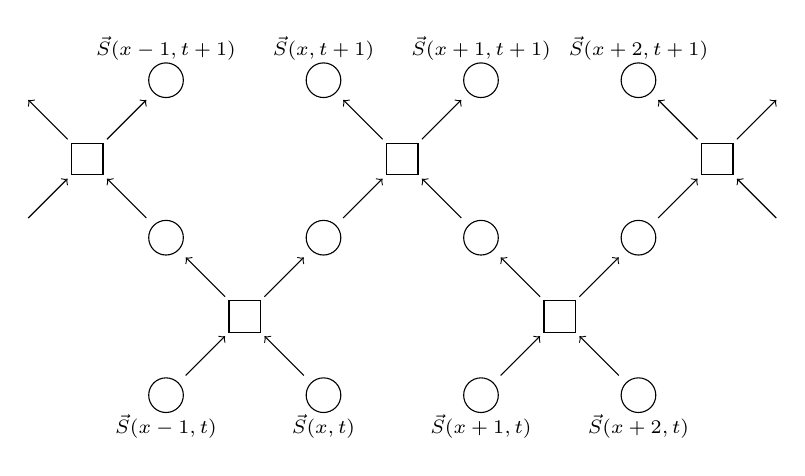
\begin{tikzpicture}[node distance = 2cm, auto, scale=1]
\spina{1}{0}{$\vec{S} (x-1,t)$}
\spina{3}{0}{$\vec{S} (x,t)$}
\spina{5}{0}{$\vec{S} (x+1,t)$}
\spina{7}{0}{$\vec{S} (x+2,t)$}
\spin{1}{2}
\spin{3}{2}
\spin{5}{2}
\spin{7}{2}
\spinb{1}{4}{$\vec{S} (x-1,t+1)$}
\spinb{3}{4}{$\vec{S} (x,t+1)$}
\spinb{5}{4}{$\vec{S} (x+1,t+1)$}
\spinb{7}{4}{$\vec{S} (x+2,t+1)$}

\interact{2}{1}
\interact{6}{1}
\interact{0}{3}
\interact{4}{3}
\interact{8}{3}

\upright{1}{0}
\upright{2}{1}
\upright{3}{2}
\upright{4}{3}
\upleft{3}{0}
\upleft{2}{1}
\upleft{1}{2}
\upright{0}{3}

\upright{5}{0}
\upright{6}{1}
\upright{7}{2}
\upleft{8}{3}
\upleft{7}{0}
\upleft{6}{1}
\upleft{5}{2}
\upleft{4}{3}

\upright{-1}{2}
\upleft{0}{3}
\upleft{9}{2}
\upright{8}{3}
% \draw[help lines] (-1,0) grid (9,4);
\end{tikzpicture}
